\chapter{Diseño}
\label{cap:capitulo4}

\begin{flushright}
\begin{minipage}[]{10cm}
\emph{En la industria, la precisión no es un lujo: es la esencia de la automatización.}\\
\end{minipage}\\

Anónimo \\
\end{flushright}

\vspace{1cm}

En este capítulo se abarca y explica el diseño completo del sistema automatizado desarrollado. En él se describen tanto los aspectos físicos de la instalación como la lógica de control implementada, abordando la selección de componentes, la configuración de la red de comunicación, y el funcionamiento de cada estación: distribución, unión y brazo robótico colaborativo. Se explican las conexiones entre los dispositivos, incluyendo los sensores, actuadores, PLCs, la interfaz HMI y el UR, así como la implementación de los distintos modos de operación mediante la Guía GEMMA, que ha servido de base para estructurar el comportamiento del sistema. Para terminar se hará un pequeño resumen del resultado final obtenido como consecuencia del trabajo realizado.

\section{Descripción general}
\label{sec:descripcion_general}

El objetivo de este trabajo es lograr que el ciclo de producción comience en la estación de distribución, donde se filtra el tipo y número de piezas que se quieren producir, después pasan a la estación unión donde se le colocará una tapa encima de las piezas bien orientadas, y finalmente, el brazo UR cogerá la pieza y la colocará en un palé para su posterior almacenamiento. 

En la sección \ref{sec:descripcion} ya se presentó una visión general del objetivo del proyecto, pero en esta se profundizará en él con una descripción más detallada y específica. El sistema global está compuesto por dos PLCs, una interfaz HMI y un robot colaborativo UR5e. Una parte fundamental del trabajo es garantizar una comunicación fluida y fiable entre todos los componentes para asegurar un funcionamiento coordinado y realista. El trabajo va a ser desarrollado en TIA portal y la comunicación via PROFINET. \\

El objetivo final es desarrollar un ciclo de producción en el que intervengan todos los componentes mencionados, simulando una aplicación industrial realista. Para ello, el ciclo debe iniciarse en la estación de distribución, donde se introducen las piezas en el proceso productivo y se identifica el tipo de material que las compone, con el fin de determinar el tratamiento correspondiente en función de sus características. Los parámetros de distinción de piezas se establecen en el HMI por el operario, si se descarta la pieza, se acabará el ciclo y se empezará de nuevo, pero si es aceptada pasará a la estación unión continuando el proceso. 

Para que la estación unión comience su proceso dentro del ciclo, es necesario que el PLC que controla la estación distribución le envíe un mensaje al segundo PLC (el que controla la estación unión) para informarle de que debe empezar.  Una vez recibido el mensaje, la segunda estación inicia el proceso tomando la pieza y deteniéndola para verificar su orientación. Si la orientación es correcta, la pieza continúa su avance en el ciclo; en caso contrario, se genera un mensaje de error en el HMI y la pieza es descartada, regresando a la estación de distribución, donde se requerirá una nueva comunicación para reiniciar el proceso. Si la pieza está bien orientada continuará su camino hasta que se pare en un punto donde la tapa proveniente de otra cinta será colocada encima de la pieza con el módulo pick \& place. Una vez terminado el ciclo la estación volverá a comunicarse con la estación unión para hacerle saber que terminó su proceso.

Una vez que el PLC de la estación unión recive el mensaje de fin de ciclo del otro PLC, el último paso es comunicarse con el UR para que termine el proceso global. El PLC asociado a la estación distribución es el encargado de mandar el mensaje vía Profinet al UR, quién iniciará una secuencia de paletizado simulando la ordenación de las piezas. Como físicamente las estaciones Festo y el UR están separadas, el proceso de paletizado del brazo robótico se realiza con bricks de leche como elemento manipulable. En el momento que el UR termine su proceso, el PLC será notificado terminando con el ciclo global y volviendo a empezar.

La función del HMI en este proyecto será proporcionar al operario una representación simplificada del sistema, permitiéndole controlarlo mediante unos pocos botones. A través de la pantalla se gestionan funciones como el inicio y la parada del sistema, la configuración del número de piezas a procesar y la selección del tipo de material permitido. Además, el HMI se utiliza para mostrar mensajes de error, como la detección de una pieza mal orientada o la notificación de que el robot UR está colocando una pieza en el palé.

\clearpage

\begin{figure}[h!]
  \begin{center}
    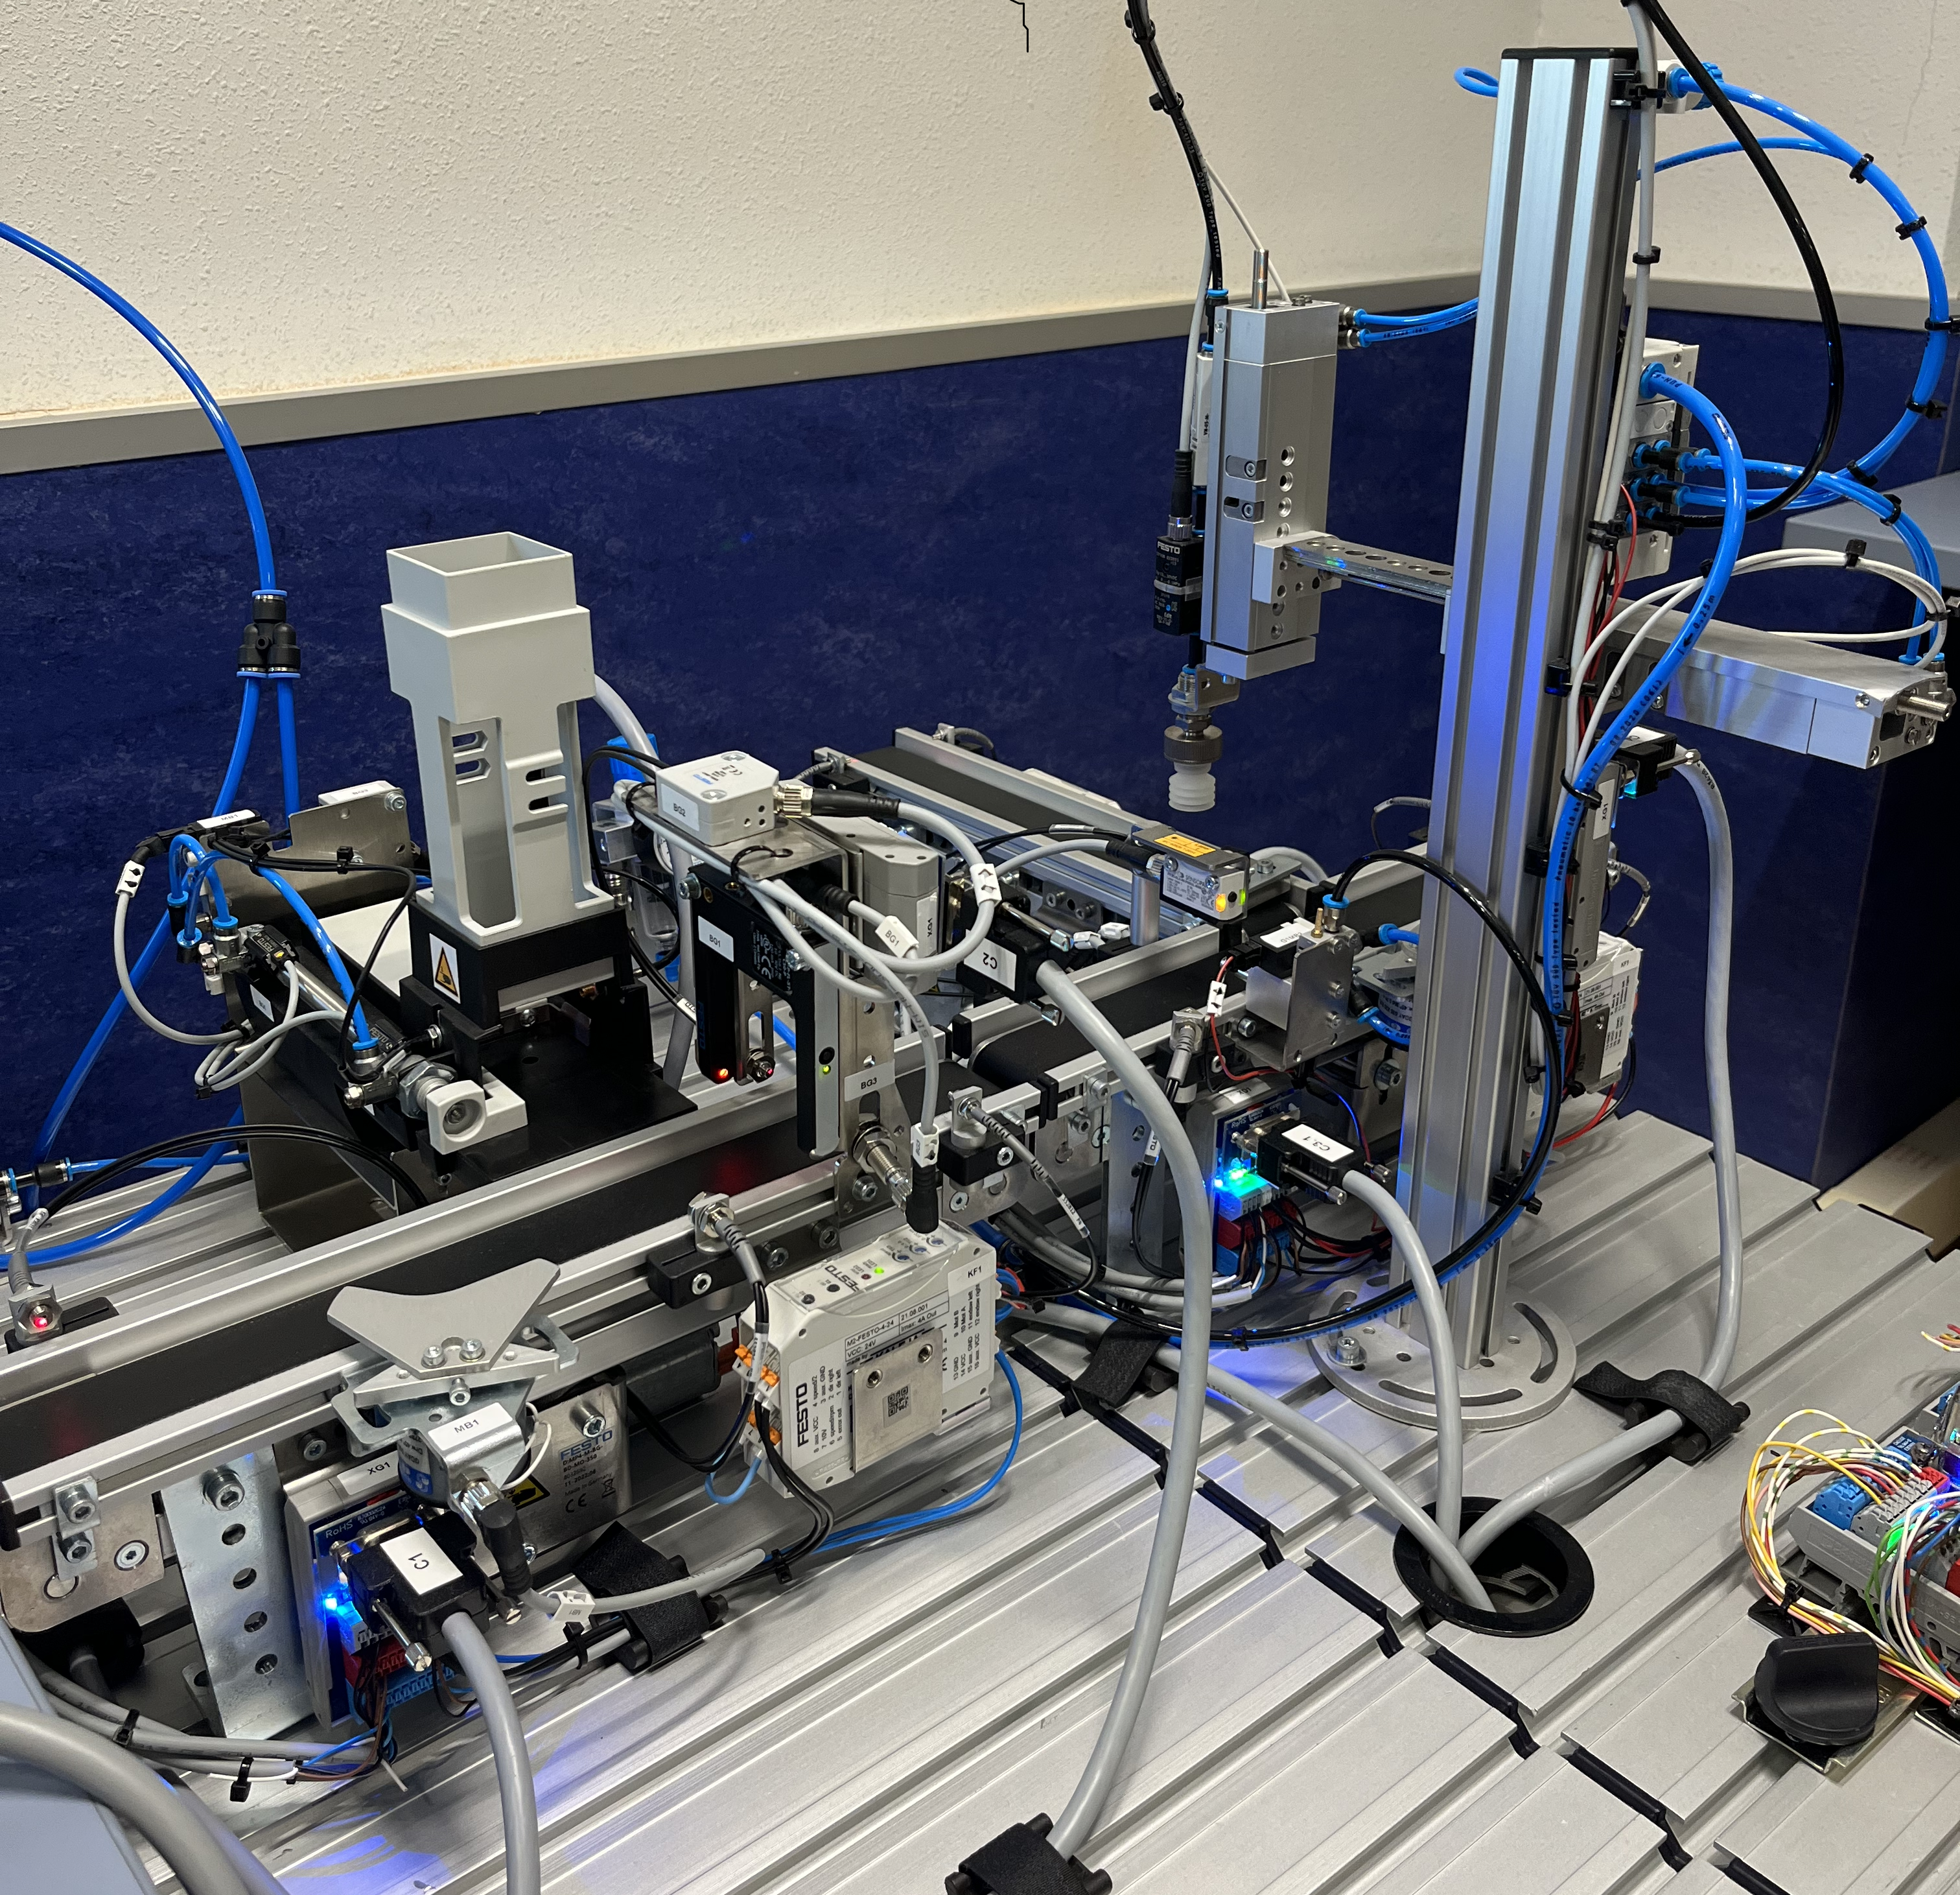
\includegraphics[width=13cm]{figs/sistemas_unidos}
  \end{center}
  \caption{\centering Estación distribución y estación unión unidas.}
  \label{fig:sistemas_unidos}
\end{figure}


\section{Conectividad de los dispositivos}
\label{sec:conectividad_dispositivos}

Para realizar la conexión de todos los dispositivos entre si, se ha utilizado el switch Ethernet industrial SCALANCE XB005 y el protocolo PROFINET, los cuales ya se ha explicado en el capítulo \ref{cap:capitulo3}. Este dispositivo cuenta con 5 puertos, soporta conexiones PROFINET y está pensado para usarse en fábricas o instalaciones automatizadas donde se requiere una red estable y confiable. El switch es ideal para el proyecto ya que se necesita comunicar 4 dispositivos más el ordenador que los programa entre ellos, ocupando los 5 puertos disponibles. Los cables Ethernet utilizados en son el modelo 6XV18703QN10 \footnote{6XV18703QN10. (n.d.). Radwell.eu. Retrieved June 10, 2025, from \url{https://www.radwell.eu/es/buy/siemens-6xv18703qn10/1018547.html}} los cuales están especialmente diseñados para este tipo de aplicaciones industriales.  \\

A continuación, se muestra un diagrama de conexiones de todos los dispositivos:

\begin{figure} [h!]
  \begin{center}
    \includegraphics[width=14cm]{figs/conexion_dispositivos}
  \end{center}
  \caption{\centering Representación de conexiones entre los dispositivos del proyecto.}
  \label{fig:conexion_dispositivos}
\end{figure} 

\begin{figure} [h!]
  \begin{center}
    \includegraphics[width=15cm]{figs/conexiones_tiaportal}
  \end{center}
  \caption{\centering Representación de conexiones entre los dispositivos dentro del proyecto de Tia Portal.}
  \label{fig:conexiones_tiaportal}
\end{figure} 

\clearpage

Para intercambiar mensajes y datos entre los dos PLCs se han utilizado las funciones de comunicación RECV y SEND. SEND permite enviar información desde un PLC a otro, mientras que RECV se encarga de recibir esos datos en el destino. Estas funciones son muy útiles para coordinar procesos distribuidos y compartir datos en tiempo real en redes como Ethernet/IP o Profinet. Para la comunicación entre los PLCs, se ha definido una estructura de datos específica para cada uno, la cual se utiliza en el intercambio de mensajes. Las estructuras mostradas en la imagen \ref{fig:estructura_com_plcs} incluyen variables booleanas utilizadas para la comunicación de tres posibles finalizaciones de ciclo, así como una variable entera que indica el tipo de pieza detectada. Contienen toda la información necesaria para el proceso, permitiendo compartir y sincronizar los datos de forma eficiente entre los distintos controladores. Cada PLC envía y recibe mensajes a una frecuencia de 5Hz y van activando o desactivando los campos de la estructura según en la etapa que se encuentren. Seguidamente se muestra una imagen de las estructuras de datos y las funciones de comunicación de los PLCs: \\

\begin{figure} [h!]
  \begin{center}
    \includegraphics[width=16cm]{figs/estructura_com_plcs}
  \end{center}
  \caption{\centering Estructuras de datos utilizadas en la comunicación entre los PLCs.}
  \label{fig:estructura_com_plcs}
\end{figure} 

\clearpage

\begin{figure} [h!]
  \begin{center}
    \includegraphics[width=10cm]{figs/comunicacion_plcs}
  \end{center}
  \caption{\centering Funciones SEND y RECV entre los PLCs.}
  \label{fig:comunicacion_plcs}
\end{figure} 

Para establecer la comunicación entre el UR y el PLC (el conectado a la estación distribución) a través de PROFINET, se ha seguido la guía oficial de UR PROFINET\footnote{Profinet Guide - 20596. (n.d.). Universal-robots.com. Retrieved June 25, 2025, from \url{https://www.universal-robots.com/articles/ur/interface-communication/profinet-how-to-guide-e-series/}}. El primer paso es activar la funcionalidad PROFINET en el UR, accediendo a la pestaña “Instalación” de este, esta acción activa un LED amarillo en el controlador, indicando que la función está habilitada pero aún no conectada. A continuación, en el entorno de programación TIA Portal, se debe actualizar la lista de dispositivos accesibles en red, y cuándo el UR aparezca en ella, se le asignan tanto la dirección IP como el nombre del dispositivo al robot. Seguidamente, se importa el archivo GSD proporcionado por Universal Robots en la misma página de la guía, que permite al TIA Portal reconocer al robot como un dispositivo PROFINET compatible. \\

Tras esto, el robot se agrega a la red en la vista de dispositivos y se enlaza con el PLC seleccionando y configurando los módulos de entrada y salida desde el catálogo que se quieren utilizar para la comunicación (en este caso todos), definiendo las direcciones de E/S. Este paso resultó ser el más complejo, ya que al principio, al escribir en direcciones de memoria incorrectas, los mensajes enviados al UR llegaban vacíos, sin embargo, tras consultar la documentación y validar la configuración, se lograron establecer las direcciones adecuadas. Las direcciones de memoria de la imagen \ref{fig:com_ur_modulos} deben coincidir con las mismas de las variables de los datos utilizadas para la comunicación representadas en la imagen \ref{fig:com_plc_ur} para poder modificar los registros de propósito general utilizados en la comunicación (las entradas empiezan en la dirección \%I100 y las salidas en la \%Q100, coincidiendo con las de las variables \texttt{UR\_IN} y \texttt{UR\_OUT}). \\

Esta configuración no fue inmediata, puesto que las guías oficiales no detallaban esta configuración de forma explícita ni proporcionaban ejemplos claros. Sin embargo, tras varios intentos y pruebas de comunicación, se intuyó que las direcciones mostradas en las figuras \ref{fig:com_ur_modulos} y \ref{fig:com_plc_ur} hacían referencia a los mismos registros del PLC, lo que permitió completar la comunicación entre estos dos dispositivos. \\

\begin{figure} [h!]
  \begin{center}
    \includegraphics[width=15cm]{figs/com_ur_modulos}
  \end{center}
  \caption{\centering Configuración de los módulos de comunicación del UR en Tia Portal.}
  \label{fig:com_ur_modulos}
\end{figure} 

\clearpage

\begin{figure} [h!]
  \begin{center}
    \includegraphics[width=13cm]{figs/com_plc_ur}
  \end{center}
  \caption{\centering Configuración de los módulos de comunicación del UR en Tia Portal.}
  \label{fig:com_plc_ur}
\end{figure} 

Finalmente, una vez que las estructuras de datos definidas por el usuario permiten mapear adecuadamente los registros de entrada y salida del robot, se pueden modificar los registros booleanos, enteros o flotantes para enviarle información desde el PLC al UR. Los datos que el PLC envía al UR se escriben en las direcciones asignadas a las salidas (UR\_OUT.Reg 1), mientras que los datos recibidos del UR se leen desde las direcciones de entrada (UR\_IN). Cuando la comunicación entre el robot y el PLC se establece con éxito, el LED del controlador del robot cambia a verde como se observa en la siguiente imagen:

\begin{figure} [h!]
  \begin{center}
    \includegraphics[width=12cm]{figs/ur_conectado_plc}
  \end{center}
  \caption{\centering Conexión establecida entre el UR y el PLC. \cite{guia_profinet}}
  \label{fig:ur_conectado_plc}
\end{figure} 

Seguidamente se muestra una tabla que resume todos los mensajes intercambiados entre los dispositivos en el ciclo global: 

\newcolumntype{M}[1]{>{\centering\arraybackslash}m{#1}}

\begin{table}[H]
\begin{center}

\renewcommand{\arraystretch}{1.5}
\begin{tabular}{|M{1.75cm}|M{1.75cm}|M{3.5cm}|M{7.5cm}|}
\hline
\textbf{Emisor} & 
\textbf{Receptor} & 
\textbf{Mensaje} & 
\textbf{Explicación} \\
\hline
PLC 1  & PLC 2 &  \makecell{Send\_fase\_1  \\ (Bool)} & Se envía si el tipo de pieza es aceptado y pasa de la estación distribución a la estación unión. \\
\hline
PLC 2  & PLC 1 &  \makecell{Send\_fase\_1  \\ (Bool)} & Confirmación de que la pieza pasó exitosamente de la estación distribución a la estación unión. \\
\hline
PLC 1  & PLC 2 &  \makecell{Tipo\_de\_pieza   \\ (Int)} &  \makecell{Indica el tipo de pieza detectado: \\ Pieza negra: 1 \\ Pieza rosa: 2 \\ pieza metálica: 3}  \\
\hline
PLC 2  & PLC 1 &  \makecell{Secuencia\_acabada  \\ (Bool)} &  Se le indica a la estación unión que la estación distribución terminó su ciclo con éxito. \\
\hline
PLC 1  & PLC 2 &  \makecell{Secuencia\_ACK   \\ (Bool)} &  Confirmación de la recepción del mensaje Secuencia\_acabada. \\
\hline
PLC 2  & PLC 1 &  \makecell{Pieza\_mal\_orientada   \\ (Bool)} &  Se le indica a la estación unión que la pieza actual está mal orientada y se debe descartar. \\
\hline
PLC 1  & PLC 2 &  \makecell{Pieza\_mal\_ACK  \\ (Bool)} &  Confirmación de la recepción del mensaje Pieza\_mal\_orientada. \\
\hline
PLC 1  & UR5e &  \makecell{Start \\ Registro GPbi [0] \\ (Bool)} & Indica el inicio de la secuencia de colocación de la pieza en el palé del UR. \\
\hline
PLC 1  & UR5e  &  \makecell{num\_capas \\ Registro GPii [0] \\ (Int)} & Número de capas elegido en el HMI que se quieren para el paletizado. \\
\hline
Ur5e  & PLC 1 &  \makecell{piezas\_paletizadas \\ Registro GPio [0] \\ (Int)} & Número de piezas paletizadas actualmente. \\
\hline
UR5e   & PLC 1 &  \makecell{ejecutando\_proc \\ Registro GPbo [0] \\ (Bool)} & Informa que el UR todavía está ejecutando su ciclo. \\
\hline
UR5e   & PLC 1 &  \makecell{pale\_completo \\ Registro GPbo [1] \\ (Bool)} & Aviso de que el palé está completo. \\
\hline
PLC 1  & UR5e  &  \makecell{pale\_recogido  \\  Registro GPbi [2] \\ (Bool)} & Informa de que el palé ha sido recogido. \\
\hline
UR5e   & PLC 1 &  \makecell{Pale\_ACK \\ Registro GPbo [2] \\ (Bool)} & Confirmación de la recepción del mensaje pale\_recogido. \\
\hline
PLC 1  & UR5e  &  \makecell{parada\_emergencia  \\  Registro GPbi [1] \\ (Bool)} & Parada de emergencia pulsada, parada obligatoria de la secuencia. \\
\hline
\end{tabular}

\caption{Intercambio de mensajes en el ciclo global del sistema.}
\label{cuadro:mensajes}
\end{center}
\end{table}
 
\section{Funcionamiento estación distribución}
\label{sec:funcionamiento_distribucion}

La estación distribución es la encargada de iniciar la secuencia del proceso automático. Está conectada al primer PLC y tiene como función principal suministrar piezas al sistema, ya sea a través de su cinta transportadora o mediante el dispensador de piezas. Además, el usuario puede seleccionar desde el HMI el tipo de material de la pieza para permitir o no su paso. También se establece un número máximo de piezas permitidas; una vez alcanzado este límite, se bloquea el paso de nuevas piezas hasta que el contador sea reiniciado, como medida de control y revisión del proceso. En caso de que la pieza no cumpla con las condiciones establecidas en la interfaz de usuario, esta será devuelta al inicio del recorrido y descartada. Si cumple los requisitos, continuará su avance hacia la siguiente estación. Adicionalmente se ha implementado un modo de prueba que permite verificar el funcionamiento individual de cada sensor y actuador, facilitando así la detección de posibles errores. A continuación, se presenta una tabla que recoge todas las entradas y salidas de la estación, así como su correspondencia con las conexiones al PLC:

\begin{table}[H]
\begin{center}

% Tabla 1 (Sensores)
\begin{tabular}{|P{6.5cm}|P{4cm}|P{2.5cm}|}
\hline
\multicolumn{1}{|c|}{\textbf{Sensor}} & 
\multicolumn{1}{c|}{\textbf{Entrada al PLC}} & 
\multicolumn{1}{c|}{\makecell{\textbf{Tipo de salida} \\ \textbf{(normalmente)}}} \\
\hline
Láser inicio cinta  & \%I0.0 &  abierta \\
Láser medio cinta  & \%I0.1 &  abierta \\
Láser final cinta  & \%I0.2 &  cerrada \\
Identificador de piezas (pieza negra)  & \%I0.4 &  abierta \\
Sensor de color (pieza rosa)  & \%I0.5 &  abierta \\
Sensor metálico (pieza metálica)  & \%I0.6 &  abierta \\
Corredera retraída  & \%I0.7 &  abierta \\
Corredera extendida & \%I1.0 &  abierta \\
Pieza en el cargador & \%I1.1 &  cerrada \\
\hline
\end{tabular}

\vspace{0.2cm}

% Tabla 2 (Actuadores)
\begin{tabular}{|P{6.95cm}|P{6.95cm}|}
\hline
\multicolumn{1}{|c|}{\textbf{Actuador}} & 
\multicolumn{1}{c|}{\textbf{Salida del PLC}} \\
\hline
Avance cinta & \%Q0.0 \\
Retroceso cinta & \%Q0.1 \\
Separador & \%Q0.2 \\
Avance corredera & \%Q0.3 \\
\hline
\end{tabular}

\caption{Entradas y salidas de la estación distribución conectadas al PLC 1}
\label{cuadro:distribucion}
\end{center}
\end{table}

El Grafcet de la figura \ref{fig:grafcet_distribucion} describe la secuencia automatizada de funcionamiento de la estación de unión. El sistema se inicializa con la variable de conteo de piezas a cero y permanece en espera hasta recibir una orden de arranque desde la interfaz HMI. En función del modo de carga seleccionado (manual o automático), se introduce la pieza en el sistema por la parte inicial de la cinta transportadora (donde será necesario activar el separador para permitir su paso) o a través de la corredera que realiza un movimiento de extensión y retracción para depositar la pieza retenida en el cargador. A continuación, se lleva a cabo una etapa de identificación en la que se determina el tipo de pieza (negra, rosa o metálica), registrándose dicha información en el sistema y actualizándose el contador de piezas correspondiente. \\

 El HMI cuenta con una interfaz para seleccionar el tipo de pieza que se quiere aceptar y la que se quiere descartar, como se observa en la imagen \ref{fig:HMI_funcionamiento}, con la configuración mostrada, los tres tipos de piezas serían descartados. Si se ha alcanzado el número total de piezas especificado por el operador o el tipo de pieza no está permitida por el operario, el sistema ejecuta un retroceso de la cinta para descartar la pieza y repetir el ciclo hasta que se reseté el contador de piezas o se amplíe el número desde el HMI. Puede haber otro caso de descarte en la estación unión, por lo que si sucede, el PLC 1 recibirá un mensaje de error procedente del PLC 2 comunicándole que le devuelve la pieza expulsándola por la zona inicial de la cinta y terminando el ciclo global. \\
 
En el caso de que no ocurra ningún imprevisto, se da por finalizado el proceso de carga de la pieza en el sistema al recibir un mensaje del PLC 2 de que la pieza pasó a su estación con éxito. Posteriormente se envía una señal al PLC 2 para confirmar la recepción de su mensaje, y a continuación, se procede a comunicarle al robot UR el inicio de su secuencia de colocación de la pieza en el palé (siempre y cuando no esté colocando ya una pieza, que en ese caso esperará a que acabe). Esta comunicación se realiza mediante la activación de un registro booleano global a través del canal PROFINET, acompañado por un registro entero que indica el número de capas de paletizado (de 1 a 4) que se quieren realizar definidas previamente en el HMI. En este punto hay dos posibles estados diferentes a los que transitar, si el UR indica que está ejecutando su secuencia, se da por terminado el ciclo global y se inicia de nuevo permitiendo comenzar el siguiente ciclo sin la necesidad de esperar a que el brazo termine su proceso. Por otro lado, si el UR indica que el palé está completo, salta un aviso en la pantalla del HMI para retirarlo como se observa en la figura \ref{fig:HMI_funcionamiento_UR_recoger} la cual ya se explicará más adelante. Tras retirar el palé, se pulsa el botón correspondiente en el HMI y, al recibir el mensaje de confirmación (ACK), el ciclo concluye.

\clearpage

\begin{figure} [h!]
  \begin{center}
    \includegraphics[width=14cm]{figs/grafcet_distribucion}
  \end{center}
  \caption{\centering Grafcet del funcionamiento de la estación distribución.}
  \label{fig:grafcet_distribucion}
\end{figure} 

En el anexo \ref{sec:anexo_distribucion} se detallan las ecuaciones lógicas del Grafcet de la estación distribución.

\clearpage

\begin{figure} [h!]
  \begin{center}
    \includegraphics[width=13.5cm]{figs/HMI_funcionamiento}
  \end{center}
  \caption{\centering Pantalla del modo funcionamiento en el HMI.}
  \label{fig:HMI_funcionamiento}
\end{figure} 


En la foto anterior se muestra la pantalla del modo funcionamiento del sistema, en la que cada botón tiene el siguiente funcionamiento:

\begin{itemize}
    \item \textbf{Número de capas:} Introducir el número de capas de paletizado deseado, siendo 1 el mínimo y 4 el máximo de capas debido a la restricción física del espacio de trabajo del cobot.
    
    \item \textbf{Número de piezas:} Introducir el número de piezas que se desean permitir en el proceso. El botón azul ``Reset `` reinicia el contador a 0.
    
    \item \textbf{Iniciar programa:} Inicia el programa después de una parada de emergencia.
    
    \item \textbf{Iniciar secuencia:} Inicia la secuencia global de producción.
    
    \item \textbf{Sólo cargador:} Indica que sólo se quieren utilizar piezas provenientes del cargador. De lo contrario, las piezas serán introducidas al sistema desde el inicio de la cinta transportadora.
    
    \item \textbf{Contador de piezas:} Muestra un contador con el número de piezas producidas hasta el momento.
    
    \item \textbf{Parada de emergencia:} Botón de seguridad que provoca que todos los elementos del proceso se paren instantáneamente.
    
    \item \textbf{Piezas Rosas:} Permite el paso de piezas rosas, de lo contrario se descartan.
    
    \item \textbf{Piezas Negras:} Permite el paso de piezas negras, de lo contrario se descartan.
    
    \item \textbf{Piezas Metálicas:} Permite el paso de piezas metálicas, de lo contrario se descartan.

\end{itemize}

\begin{figure}[h!]
  \begin{center}
  	\includegraphics[width=15cm]{figs/HMI_funcionamiento_UR_recoger}
  \end{center}
  \caption{\centering Botón utilizado para la confirmación de que el palé ha sido recogido en la pantalla de funcionamiento del HMI.}
  \label{fig:HMI_funcionamiento_UR_recoger}
\end{figure}

En la figura anterior se presenta una captura de pantalla del HMI en modo de funcionamiento, mostrando un mensaje que indica que el UR está colocando la \textbf{última pieza} del palé, parando el resto del sistema hasta que le botón ``Palé recogido'' sea pulsado. Al pulsar este botón, y siempre que el UR haya finalizado correctamente la colocación de dicha pieza, se envía una señal de confirmación al brazo robótico para verificar que el palé ha sido recogido de forma segura. Esto permite que la producción continúe sin interrupciones, garantizando la coordinación y seguridad en la línea de ensamblaje.

\clearpage

\section{Funcionamiento estación unión}
\label{sec:funcionamiento_union}

La estación de unión es la encargada de ensamblar las diferentes piezas que llegan desde la estación anterior, la cual se encuentra conectada al segundo PLC del sistema y tiene como objetivo principal la unión de una base con una tapa, verificando previamente que ambas piezas estén correctamente posicionadas. El proceso de unión se lleva a cabo mediante un actuador neumático equipado con una ventosa, el cual puede desplazarse entre las dos cintas transportadoras para ascender o descender con el fin de recoger o depositar las tapas. En caso de que alguna de las piezas se encuentre mal posicionada, el sistema detiene el ciclo, notifica el error a través de un mensaje mostrado en la pantalla del HMI y descarta la pieza afectada. Esta estación, al igual que la estación de distribución, dispone de un modo de prueba que permite revisar de forma individual el funcionamiento de cada sensor y actuador, lo cual facilita la identificación de posibles fallos. A continuación, se presentan la tabla \ref{cuadro:union}, en la que se detallan todas las entradas y salidas de la estación, así como su correspondiente conexión con el PLC.

\begin{table}[H]
\begin{center}

% Tabla 1 (Sensores)
\begin{tabular}{|P{6.5cm}|P{4cm}|P{2.5cm}|}
\hline
\multicolumn{1}{|c|}{\textbf{Sensor}} & 
\multicolumn{1}{c|}{\textbf{Entrada al PLC}} & 
\multicolumn{1}{c|}{\makecell{\textbf{Tipo de salida} \\ \textbf{(normalmente)}}} \\
\hline
Láser inicio cinta 1 & \%I0.0 &  abierta \\
Láser medio cinta 1  & \%I0.1 &  abierta \\
Láser final cinta 1  & \%I0.2 &  cerrada \\
Orientación correcta  & \%I0.3 &  abierta \\
Láser final cinta 2 & \%I0.4 &  abierta \\
Láser inicio cinta 2 & \%I0.5 &  cerrada \\
Carro retraído & \%I0.6 &  abierta \\
Carro extendido & \%I0.7 &  abierta \\
Ventosa arriba & \%I1.0 &  abierta \\
Pieza succionada & \%I1.1 &  abierta \\

\hline
\end{tabular}

\vspace{0.2cm}

% Tabla 2 (Actuadores)
\begin{tabular}{|P{6.95cm}|P{6.95cm}|}
\hline
\multicolumn{1}{|c|}{\textbf{Actuador}} & 
\multicolumn{1}{c|}{\textbf{Salida del PLC}} \\
\hline
Avance cinta 1 & \%Q0.0 \\
Retroceso cinta  2 & \%Q0.1 \\
Extender separador & \%Q0.2 \\
Retraer tope & \%Q0.3 \\
Avance cinta 2 & \%Q0.4 \\
Retroceso cinta 2 & \%Q0.5 \\
Retroceso carro & \%Q0.6 \\
Avance carro & \%Q0.7 \\
Bajar ventosa & \%Q1.0 \\
Vacío conectado & \%Q1.1 \\
\hline
\end{tabular}

\caption{Entradas y salidas de la estación unión conectadas al PLC 2}
\label{cuadro:union}
\end{center}
\end{table}

El Grafcet de la estación distribución se muestra en la figura \ref{fig:grafcet_union}, cuyo proceso inicia activando el avance de la cinta 1 al recibir un mensaje del PLC 1 hasta que la pieza proveniente de la estación distribución es detectada por el láser del inicio, luego se envía un mensaje de confirmación de que la pieza llegó al segundo sistema. La cinta continúa moviéndose hasta que la pieza es detectada en el centro de la cinta por el segundo láser y se extiende el retenedor para poder así comprobar correctamente la orientación de la pieza. A continuación se verifica la orientación de la pieza utilizando un sensor capacitivo: si la pieza está correctamente orientada, el sensor no la detecta, mientras que si está invertida, el sensor la activa, indicando una orientación incorrecta. Hay que tener en cuenta que si se trata de una pieza metálica, el sensor tiene el comportamiento opuesto, detectándose en caso de que esté correctamente orientada, por lo que en el Grafcet se han tenido que establecer las condiciones específicas para las piezas de este material. Si se confirma que la orientación es válida, paralelamente se dan dos sucesos: en el primero se vuelve a activar la cinta 1, se extiende el derivador y se espera el tiempo necesario para que la pieza llegue hasta este último y el segundo consiste en que la cinta 2 avanza hasta que en el láser del inicio de esta detecta una tapa. \\

Una vez la pieza está parada y la tapa lista para recogerse, el carro se extiende, desciende la ventosa, succiona la pieza, se eleva y se retrae colocándola encima. Después la ventosa se desactiva, se activa la cinta 1 nuevamente y se retrae el separador permitiendo a la pieza llegar al final de la cinta, que, cuando es detectada por el último láser, manda un mensaje al PLC 1 indicando que la secuencia ha terminado. Si la orientación es incorrecta, se activa un proceso de rechazo y una notificación al operario en el HMI mostrando un mensaje y contador de piezas defectuosas. El sistema esperará hasta que el operario pulse el botón de “descartar pieza” como se ve en la imagen \ref{fig:HMI_descarte}. Una vez pulsado, se activa el retroceso de la cinta y el envío de un mensaje de error al PLC 1 avisando que debe descartar la pieza. El ciclo finaliza tras la confirmación de recepción de la secuencia completada o de pieza defectuosa por parte del PLC 1.

\clearpage
 
 \begin{figure}[h!]
  \includegraphics[width=15cm]{figs/grafcet_union}
  \caption{\centering Grafcet de funcionamiento de la estación unión.}
  \label{fig:grafcet_union}
\end{figure}

En el anexo \ref{sec:anexo_union} se detallan las ecuaciones lógicas del Grafcet de la estación distribución.

\clearpage

\begin{figure}[h!]
  \includegraphics[width=15cm]{figs/HMI_descarte}
  \caption{\centering Aviso de pieza defectuosa en el modo funcionamiento en el HMI.}
  \label{fig:HMI_descarte}
\end{figure}

\section{Aplicación de la Guía GEMMA}
\label{sec:aplicacion_gemma}

La aplicación de la Guía GEMMA, explicada previamente en la sección \ref{sec:terceraseccion}, representa un elemento clave en el desarrollo de sistemas automatizados, especialmente en entornos industriales. En el contexto del proyecto, la Guía GEMMA ha sido de gran utilidad para estructurar de forma lógica y ordenada las distintas acciones que componen el ciclo global de producción. Gracias a su enfoque, ha sido posible identificar de manera precisa las condiciones iniciales, las etapas activas del proceso y las posibles interrupciones. Esta clasificación favorece la implementación de programas más robustos y fácilmente mantenibles, además de mejorar la comprensión del funcionamiento general del sistema por parte de otros desarrolladores o técnicos. Para su correcta aplicación, se han definido y utilizado en el proyecto los siguientes estados operativos:

\begin{table}[H] 
\begin{center}

\renewcommand{\arraystretch}{1.5}
\begin{tabular}{|P{3.5cm}|P{4cm}|P{7cm}|}
\hline
\textbf{Modo} & \textbf{Tipo} & \textbf{Objetivo} \\
\hline

\multirow{2}{=}{Proceso de funcionamiento} 
    & F1: Producción normal & Se realizan las tareas principales del sistema. \\
\cline{2-3}
    & F4: Marchas de verificación sin orden & Se realiza un control manual de los actuadores y la comprobación del funcionamiento de los sensores. \\
\hline

\multirow{3}{=}{Proceso de parada o puesta en marcha} 
    & A1: Parada en el estado inicial & Estado de reposo de la máquina. \\
\cline{2-3}
    & A2: Parada solicitada al final de ciclo & Estado al que se llega  cuando se termina el ciclo y pasa al estado inicial\\
\cline{2-3}
    & A3: Parada solicitada en un estado determinado & Estado al que llega la máquina alternativo el cual no coincide con el final de ciclo. \\
\cline{2-3}
    & A4: Parada obtenida & Estado de reposo diferente al principal. \\
\cline{2-3}
    & A5: Puesta en marcha después de defecto & Estado posterior a un defecto y necesario para restablecer el sistema. \\
\hline

Proceso en defecto & D1: Parada de emergencia & Estado al que llega el sistema tras una parada de emergencia. Se para el funcionamiento de todo el sistema. \\
\hline

\end{tabular}

\caption{Estados de la Guía GEMMA utilizados en el sistema.}
\label{cuadro:union}
\end{center}
\end{table}

\subsubsection{Proceso de funcionamiento}

En el proceso de funcionamiento hay configurados dos estados distintos, El primer estado es el F1 o producción normal, estado en el que el sistema repite constantemente el ciclo de producción que ha sido programado. En este estado y como se puede observar en la figura \ref{fig:HMI_funcionamiento}, se pueden configurar los parámetros del sistema desde el HMI con aspectos clave como: seleccionar el tipo de pieza que se quiere dejar pasar, introducir el número de piezas que se quieren producir,  iniciar o parar la secuencia o decidir si se quiere utilizar el cargador o no. El sistema estará dentro de este estado principal, siempre y cuando no surja algún imprevisto o comportamiento extraño.

En cuanto al estado F4 o marcha de verificación sin orden, tiene como objetivo realizar un control manual de los actuadores y sensores para comprobar su correcto funcionamiento. Para este estado se han creado dos modos de test a cada estación física (distribución y unión, Estos modos de pruebas son seleccionables en el menú principal del HMI antes de entrar en el estado de producción F1 como se aprecia en la imagen \ref{fig:HMI_inicio}. Una vez dentro del modo test, y por lo tanto, dentro del estado F4, se puede acceder a una vista de diagnóstico de errores general o  se puede escoger entre el modo de pruebas de la estación distribución o unión. La estación distribución sólo cuenta con un modo test, en cambio la estación unión cuenta con dos modos debido a que tiene más sensores y actuadores para probar el funcionamiento.

\begin{figure}[H]
  \centering

  \begin{minipage}{0.8\textwidth}
    \centering
    \includegraphics[width=\textwidth]{figs/HMI_inicio}
    \captionof{figure}{\centering Estado inicial del HMI.}
    \label{fig:HMI_inicio}
  \end{minipage}
  \hfill
  \begin{minipage}{0.8\textwidth}
    \centering
    \includegraphics[width=\textwidth]{figs/HMI_test_principal}
    \captionof{figure}{\centering Vista del HMI dentro de la opción Modo Test.}
    \label{fig:HMI_test_principal}
  \end{minipage}

\end{figure}
\clearpage

En la figura \ref{fig:HMI_test_distribucion} se pueden ver todos los test que se le pueden realizar en la estación distribución. Es posible activar y desactivar manualmente los actuadores del sistema, como la cinta transportadora, el separador o el cargador, con el fin de verificar su correcto funcionamiento. Además, se muestran tres columnas y tres filas de círculos que representan visualmente todos los sensores de la estación de distribución, así como el tipo de pieza detectado por el módulo adicional de dicha estación. Cuando un sensor está activo, su indicador aparece en verde; en caso contrario, se muestra en rojo. En cuanto al tipo de pieza, solo se activa el correspondiente al detectado durante el ciclo de trabajo en curso. Esta visualización facilita la comprobación del estado de los sensores y permite monitorizar el proceso para detectar posibles errores como se muestra en la siguiente imagen: 

\begin{figure}[h!]
  \begin{center}
  	\includegraphics[width=12cm]{figs/HMI_test_distribucion}
  \end{center}
  \caption{\centering Visualización del modo Test de la estación distribución dentro del HMI.}
  \label{fig:HMI_test_distribucion}
\end{figure}

Por otro lado, el modo test de la estación de unión se ha distribuido en dos pantallas distintas, ya que el elevado número de sensores y actuadores impide representarlos todos de forma clara en una sola vista. La estructura de este modo sigue el mismo esquema que en la estación de distribución: se emplean botones para activar o desactivar los actuadores, y se utilizan círculos de colores para indicar visualmente el estado de los sensores. Un círculo verde señala un sensor activo, mientras que el rojo indica que está desactivado y también se cuenta con un botón que al presionarlo el HMI abre la pantalla del otro test programado para esta estación. A continuación se muestra el modo test para la estación unión:

\begin{figure}[H]
  \centering

  \begin{minipage}{0.95\textwidth}
    \centering
    \includegraphics[width=\textwidth]{figs/HMI_test_union_1}
    \captionof{figure}{\centering Vista del HMI dentro de la opción Modo Test 1 de la estación unión.}
    \label{fig:HMI_test_union_1}
  \end{minipage}
  \hfill
  \begin{minipage}{0.95\textwidth}
    \centering
    \includegraphics[width=\textwidth]{figs/HMI_test_union_2}
    \captionof{figure}{\centering Vista del HMI dentro de la opción Modo Test 2 de la estación unión.}
    \label{fig:HMI_test_union_2}
  \end{minipage}
\end{figure}


\subsubsection{Proceso de parada o puesta en marcha}

Este conjunto de estados definidos por la Guía GEMMA describe las distintas situaciones en las que una máquina puede encontrarse durante la detención o reactivación del proceso. Son fundamentales para garantizar transiciones seguras y controladas entre ciclos de funcionamiento. A continuación, se explican los cuatro estados que componen este proceso:

\begin{itemize}
    \item \textbf{A1: Parada en el estado inicial} \\
    Representa el estado de reposo principal de la máquina. Es el punto de partida al que se regresa tras completar un ciclo \cite{guia_gemma}. En este estado, no hay procesos activos y la máquina está lista para comenzar un nuevo ciclo de forma segura una vez se pulse dentro de la interfaz del HMI el botón ``Iniciar secuencia''.

    \item \textbf{A2: Parada solicitada al final de ciclo} \\
    Este estado funciona como transición entre la producción normal del sistema a la parada del estado inicial cuando se termina el ciclo principal \cite{guia_gemma}. Cada vez que el sistema termina su ciclo, se queda parado y transiciona al estado A1 de forma automática para volver a empezar la secuencia. Esta parada permite volver al estado inicial de parada una vez ha terminado el ciclo de producción si no está activado el botón ``iniciar secuencia'' en el HMI, permitiendo así parar el ciclo de producción.
    
    \item \textbf{A3: Parada solicitada en un estado determinado} \\
    Corresponde a una parada anticipada, en un punto concreto del ciclo, distinto del final \cite{guia_gemma}. Se emplea cuando es necesario interrumpir el proceso en un estado específico, por razones de control, mantenimiento o condiciones externas \cite{guia_gemma}. Este estado se alcanza cuando le llega a la estación unión una pieza mal orientada, por lo que el estado se queda detenido hasta que el operario descarta la pieza en el HMI, la imagen \ref{fig:HMI_descarte} representa este estado. También existe otra forma de alcanzar este estado, la cual ocurre cuando el UR ha colocado la última pieza del palé y el sistema queda en espera hasta que el operario retire el palé manualmente. Posteriormente, el operario debe pulsar el botón “palé recogido” para que el proceso continúe, tal como se muestra en la figura \ref{fig:HMI_funcionamiento_UR_recoger}. \\

    \item \textbf{A4: Parada obtenida} \\
    Indica que la máquina ha alcanzado un estado de reposo diferente al inicial A1 y proveniente del A3 \cite{guia_gemma}. Este estado alternativo está asociado a situaciones específicas, como pruebas, diagnóstico o pausas no planificadas \cite{guia_gemma}. Esta parada se activa al cumplirse cualquiera de las dos condiciones descritas en el estado A3, ambas necesarias para garantizar un funcionamiento seguro y correcto del sistema.
    
   \item \textbf{A5: Puesta en marcha después de defecto} \\
   En este estado se realizan las acciones necesarias para la reanudación del correcto funcionamiento del sistema después de un defecto \cite{guia_gemma}. \\
   A este estado se llegará después de una parada de emergencia y será necesario pulsar el botón ``iniciar programa'' en la interfaz HMI de modo funcionamiento para transicionar al estado A1.
\end{itemize}

\subsubsection{Proceso en defecto}

Dentro del proceso de defecto sólo se ha programado el estado D1 de parada de emergencia. Este estado representa una situación crítica en la que el sistema se detiene de forma inmediata debido a una emergencia \cite{guia_gemma}. La parada se realiza sin esperar a que finalice el ciclo, con el objetivo de garantizar la seguridad de las personas, del sistema o del entorno \cite{guia_gemma}. Este estado puede ser alcanzado en cualquier momento que se presione el botón ``parada de emergencia'' desde el HMI en el modo de funcionamiento. Una vez pulsado el botón se para el funcionamiento de todo el sistema para ser revisado por un operario, y una vez resuelto el problema, se podrá volver a comenzar con el ciclo de producción desde 0.

\subsubsection{Aplicación de la Guía GEMMA}

Una vez descritos en detalle todos los posibles estados que puede adoptar el sistema a lo largo de su funcionamiento, se presenta a continuación la imagen \ref{fig:guia_gemma_final} muestra gráficamente todas las transiciones entre dichos estados. Esta representación visual resulta especialmente útil para comprender de forma global el comportamiento del sistema automatizado en sus distintas fases operativas. 

\clearpage

\begin{figure}[h!]
  \begin{center}
  	\includegraphics[width=16.5cm]{figs/guia_gemma_final}
  \end{center}
  \caption{\centering Esquema de transiciones de la aplicación de la Guía GEMMA en el sistema.}
  \label{fig:guia_gemma_final}
\end{figure}

En la figura, los elementos de color verde corresponden al proceso de funcionamiento normal, los de color amarillo al proceso de parada o de puesta en marcha, y los de color rojo al proceso de detección de defectos o fallos. La imagen también cuenta con una leyenda explicando las acciones necesarias para transicionar entre estados.

\clearpage

\section{Funcionamiento cobot UR5e}
\label{sec:funcionamiento_ur5e}

El cobot UR5e es un brazo robótico colaborativo diseñado para trabajar de forma segura junto a operarios. En este proyecto, su función principal es comunicarse con los PLCs para ejecutar una secuencia de paletizado en la fase final del ciclo global del sistema. Una vez que la estación de unión completa su ciclo, el PLC 1 envía una señal al UR5e indicándole que inicie su secuencia. Al finalizar la operación de colocación de la pieza en el palé, el cobot notifica al PLC 1 que ha concluido, permitiendo así reiniciar el ciclo completo. El propósito de integrar el brazo en la ejecución del sistema es simular su uso dentro del proceso automático (aunque físicamente no se pudo integrar debido a la distancia entre estaciones) para ordenar las piezas , aportando así mayor realismo y complejidad al resultado final. 

El cobot viene equipado con una pinza neumática como herramienta. Esta pinza permite sujetar, mover y soltar objetos de forma rápida y eficiente. Es ideal para tareas repetitivas como ensamblaje, paletizado, manipulación de piezas o carga de máquinas, especialmente cuando no se requiere un control preciso de la fuerza. Esta pinza se ha utilizado para la secuencia de paletizado, la cual sigue el esquema llamado \textbf{paletizado por capas}. Este tipo de paletizado por capas consiste en organizar productos sobre un palé formando niveles horizontales uniformes agrupando varios elementos alineados o alternos para lograr estabilidad \cite{paletizado_capas}. Es ideal para cargas regulares y facilita la automatización, optimizando espacio, transporte y manipulación en entornos industriales \cite{paletizado_capas}. 

\begin{figure}[h!]
  \begin{center}
  	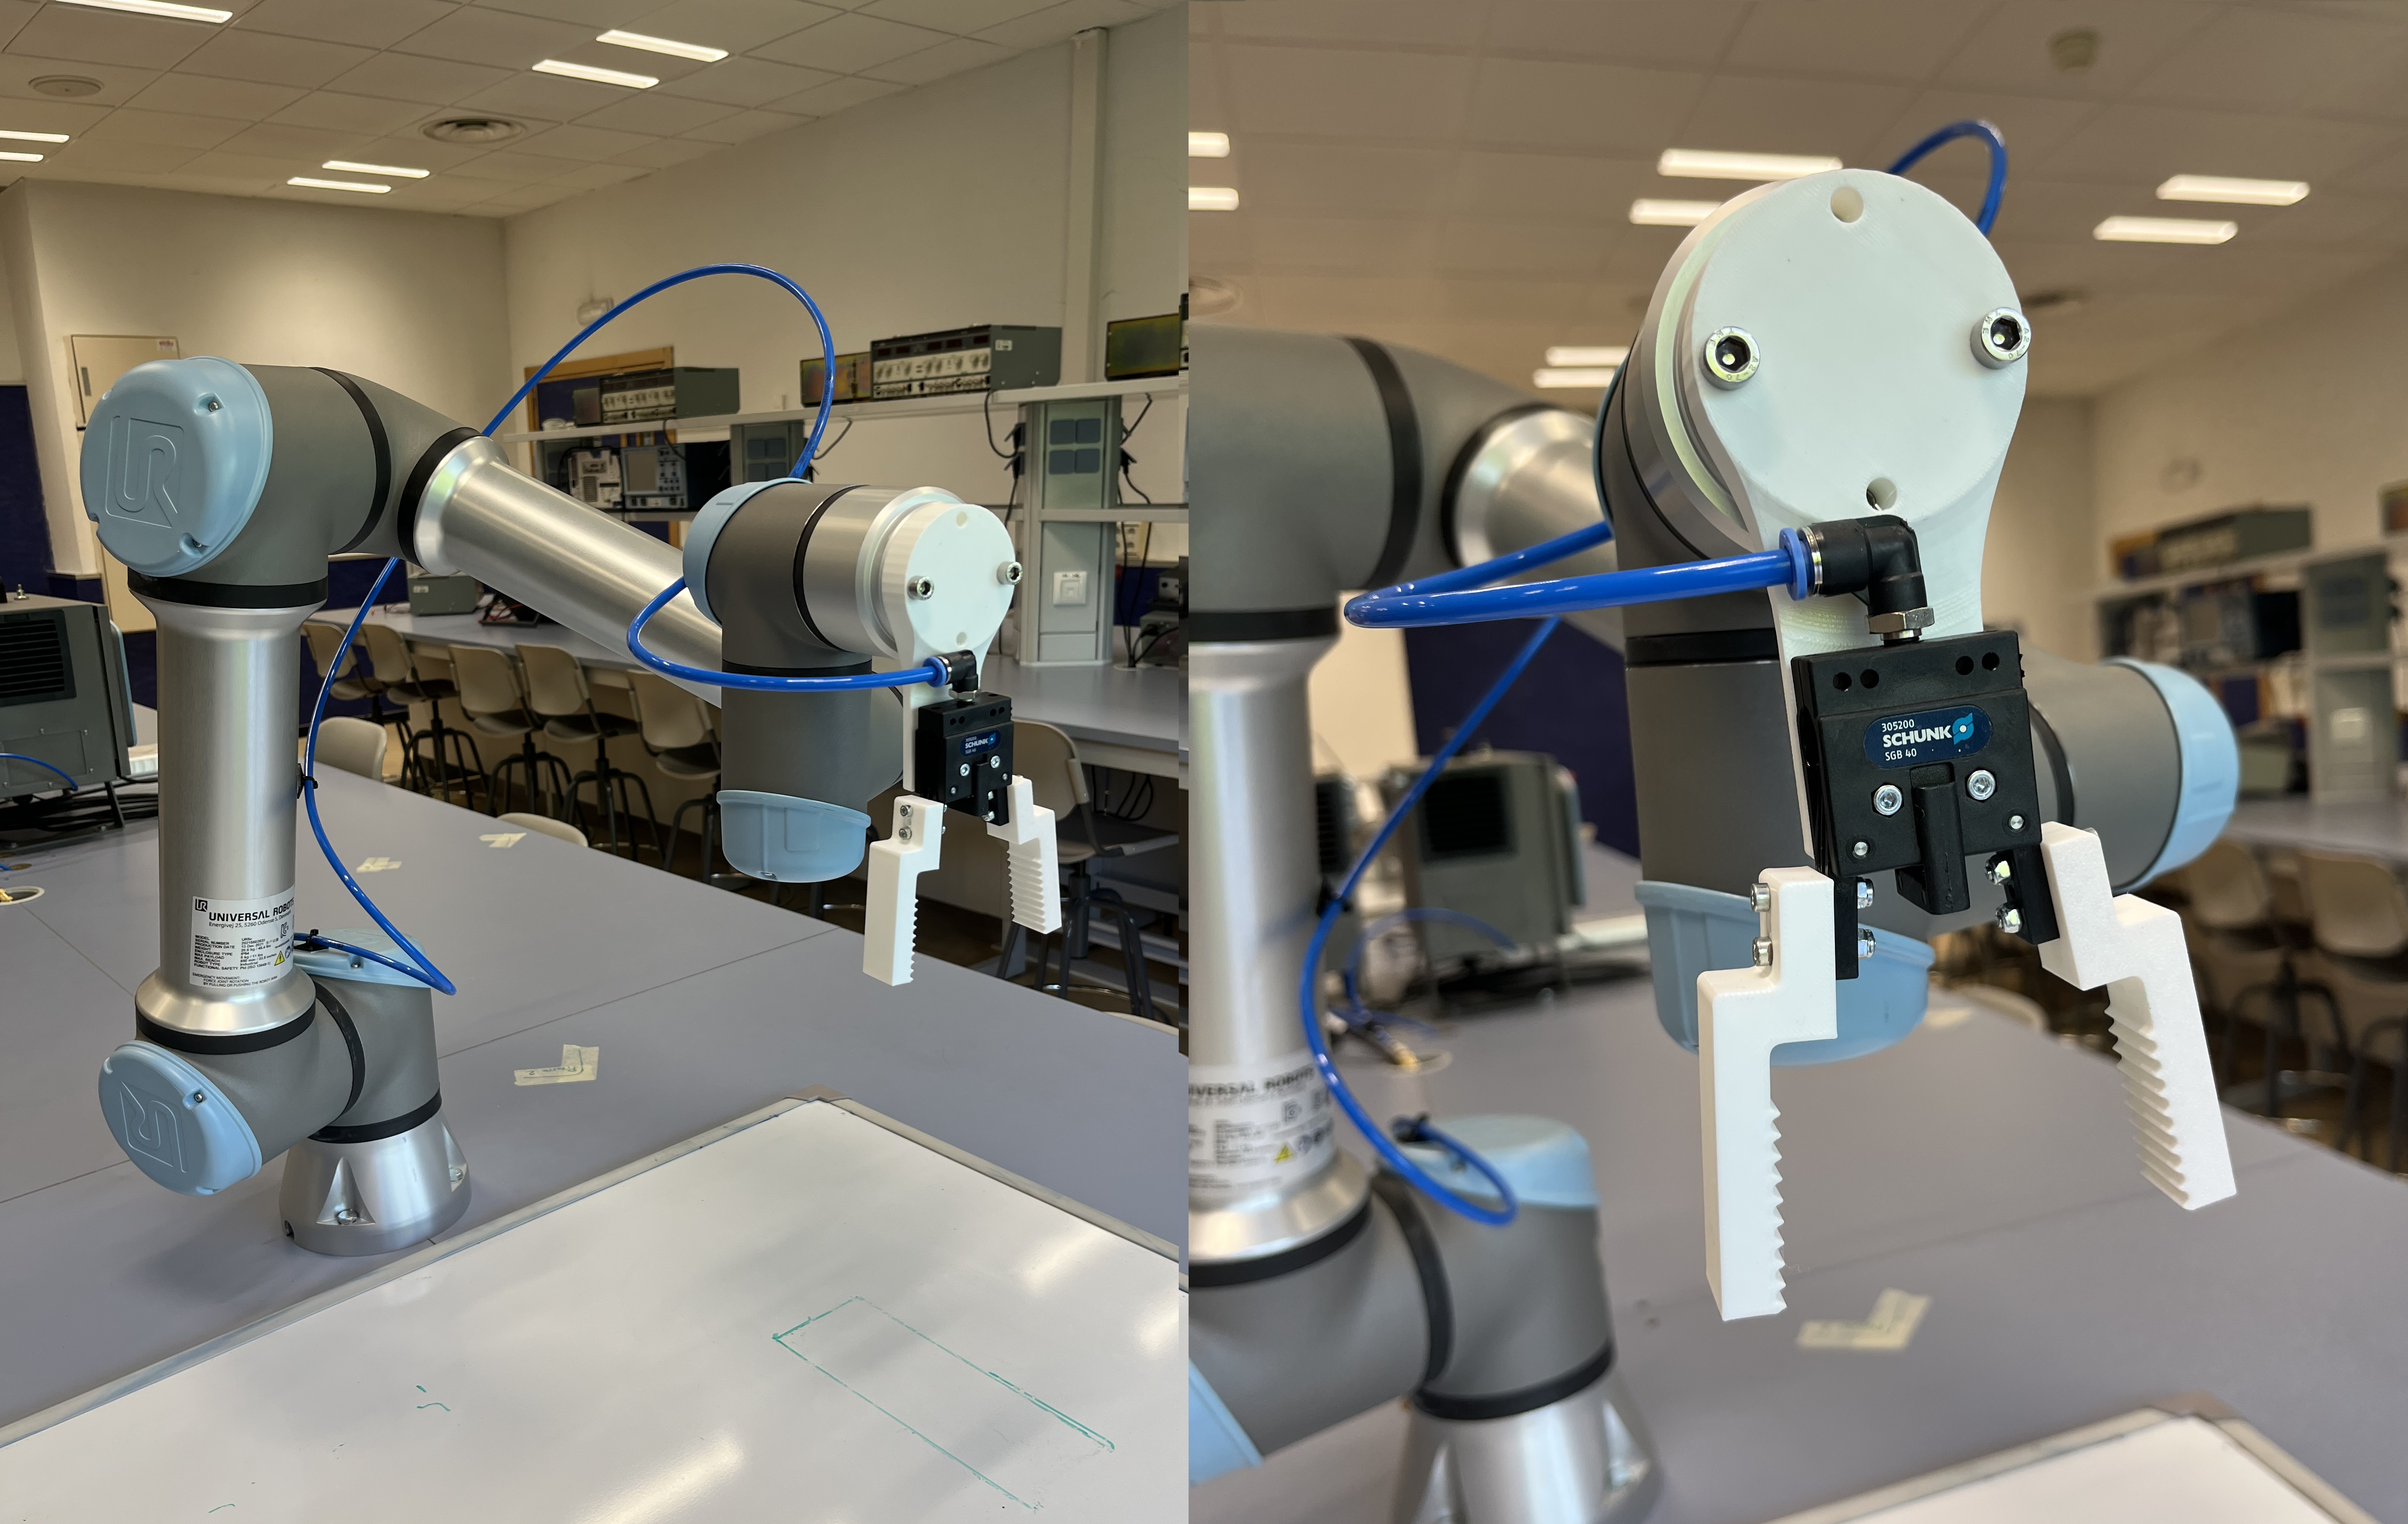
\includegraphics[width=11.5cm]{figs/brazo_pinza}
  \end{center}
  \caption{\centering UR5e junto con la pinza como herramienta.}
  \label{fig:brazo_pinza}
\end{figure}

Como ya se ha visto en la sección \ref{sec:conectividad_dispositivos}, el PLC 1 le envía un mensaje al UR para iniciar el programa de paletizado. En este programa se ha utilizado la herramienta de paletizado integrada en Polyscope. Esta funcionalidad permite crear un palé de cualquier tipo de elemento indicando únicamente el número de capas deseadas y las coordenadas de la posición de cada uno. Tal como se ha mencionado anteriormente, se ha llevado a cabo un paletizado por capas, utilizando bricks de leche como elementos a colocar, simulando una secuencia real en un entorno industrial. Se han configurado cuatro capas en total: dos con una disposición determinada y las otras dos con una diferente, obteniendo el siguiente resultado:

\begin{figure}[h!]
  \begin{center}
  	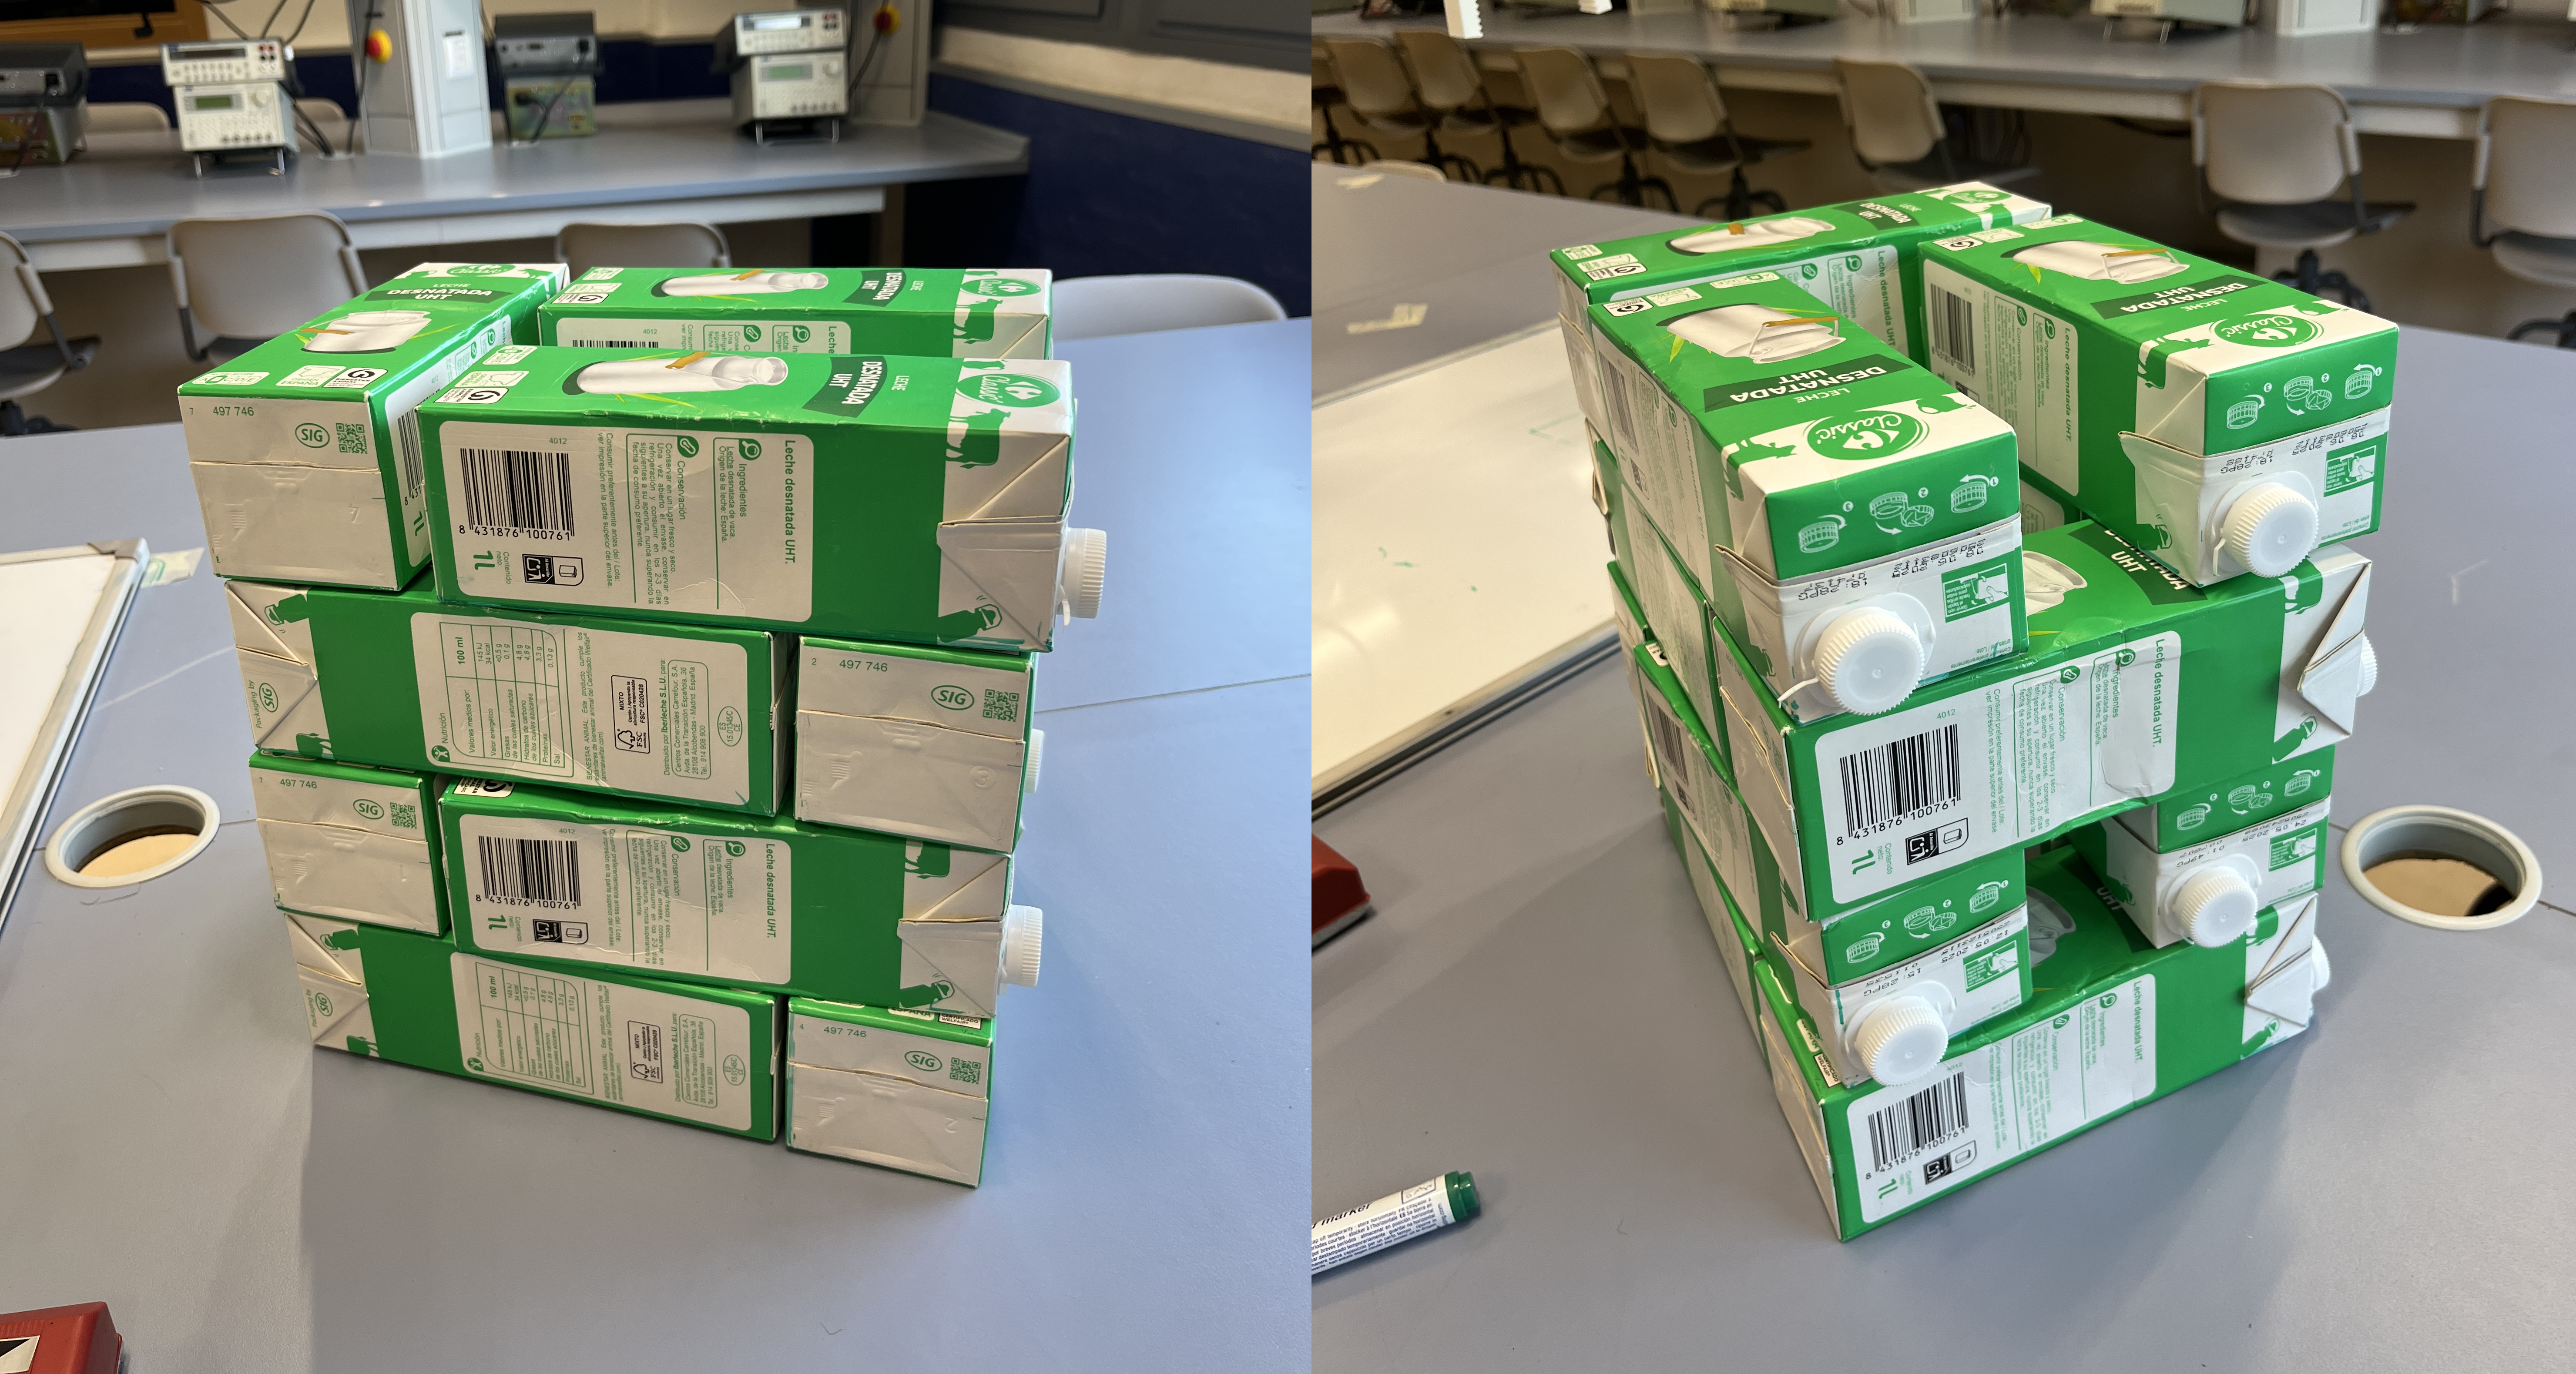
\includegraphics[width=14.5cm]{figs/resultado_paletizado}
  \end{center}
  \caption{\centering Resultado final del paletizado de bricks de leche por el UR5e.}
  \label{fig:resultado_paletizado}
\end{figure}

Las coordenadas de la posición de las piezas en el paletizado se han tomado de forma relativa a la coordenada del primer brick de leche. La primera coordenada se definió en la posición que se quería colocar el primer elemento del palé, y a partir de esta y tomándola de referencia, se han definido las 5 coordenadas restantes. Al utilizar el sistema de coordenadas del primer punto se han podido colocar elementos paralelos y perpendiculares al primero, ayudando a aportar gran estabilidad y orden al palé. Esta técnica también ha ayudado mucho a establecer la misma altura de todos los bricks de leche y asegurarse así que no se coloquen de forma uniforme. Adicionalmente, se han establecido algunos puntos de paso también utilizando este sistema de coordenadas para intentar establecer los movimientos lo más rectilíneos posibles. Seguidamente se muestra una tabla que refleja las coordenadas de las posiciones de cada pieza que forman el palé, tomando como referencia la primera posición para definir el resto de ellas:

\begin{table}[H]
\begin{center}

\renewcommand{\arraystretch}{1.5}
\begin{tabular}{|M{2.45cm}|M{2.65cm}|M{1.2cm}|M{1.2cm}|M{1.2cm}|M{1.1cm}|M{1.1cm}|M{1.1cm}|}
\hline
\textbf{Coordenada de la pieza} &
\textbf{Sistema de coordenadas} & 
\textbf{X (mm)} & 
\textbf{Y (mm)} & 
\textbf{Z (mm)} &
\textbf{RX (rad)} &
\textbf{RY (rad)} &
\textbf{RZ (rad)} \\
\hline
Posición 1  & Base UR5e &  -333,6 & 270,9 & 70,0 & 0 & 3,15 & 0 \\
\hline
Posición 2  & Posición 1 &  0 & -128 & 0 & 0 & 0 & 0 \\
\hline
Posición 3  & Posición 1 &  198,3 & -82,3 & 0 & 0 & 0 & 1,57 \\
\hline
Posición 4  & Posición 1 &  -43,3 & -24,8 & 0 & 0 & 0 & 4,71 \\
\hline
Posición 5  & Posición 1 &  90 & 0 & 0 & 0 & 0 & 0 \\
\hline
Posición 6  & Posición 1 &  90 & -128 & 0 & 0 & 0 & 0 \\
\hline
\end{tabular}

\caption{\centering Coordenadas de colocación de las piezas en el palé utilizando el UR5e.}
\label{cuadro:coordenadas}
\end{center}
\end{table}

En cuanto a la comunicación PROFINET entre el UR y el PLC 1 ya explicada en la sección \ref{sec:conectividad_dispositivos}, se han utilizado los siguientes registros de propósito general para el intercambio de información en los mensajes entre ambos:

\begin{table}[H]
\begin{center}

\renewcommand{\arraystretch}{1.5}
\begin{tabular}{|M{3.4cm}|M{2.3cm}|M{3cm}|M{2.5cm}|M{2cm}|}
\hline
\textbf{Nombre variable} &
\textbf{Número de registro} & 
\textbf{Direcci\'on para el UR5e} & 
\textbf{Direcci\'on para el PLC} &
\textbf{Tipo de dato} \\
\hline
Start  & GPbi [0] & Entrada & Salida & Bool \\
\hline
parada\_emergencia  & GPbi [1] & Entrada & Salida & Bool \\
\hline
pale\_recogido  & GPbi [2] & Entrada & Salida & Bool \\
\hline
num\_capas  & GPii [0] & Entrada & Salida & Int \\
\hline
piezas\_paletizadas  & GPio [0] & Salida & Entrada  & Int \\
\hline
ejecutando\_proc  & GPbo [0] & Salida & Entrada & Bool \\
\hline
pale\_completo  & GPbo [1] & Salida & Entrada & Bool \\
\hline
pale\_ACK  & GPbo [2] & Salida & Entrada & Bool \\
\hline

\end{tabular}

\caption{Registros utilizados para la comunicación entre el UR5e y el PLC 1.}
\label{cuadro:registros}
\end{center}
\end{table}

En el cuadro \ref{cuadro:mensajes} ya se ha explicado el objetivo y significado de la utilización de estos registros en el código del UR; sin embargo, en este apartado se va a profundizar aún más en su funcionamiento, describiendo detalladamente la lógica implementada, comentando el código del brazo robótico que se muestra a continuación, y explicando cómo se gestionan las señales de comunicación y sincronización de tareas.

\begin{code}[h]
\begin{lstlisting}[]
# AntesDeIniciar
Ajustar ejecutando_proc= False
capa_controller := 0
contador_piezas := 0
num_capas := numero_capas*3
if num_capas>12
    num_capas:=12

# Programa de robot
Bucle num_capas>contador_piezas:
    Ajustar pale_completo= False
    Ajustar pale_ACK= False
    Moverj
        Punto_inicio
    # Esperar al mensaje de inicio del PLCs
    Esperar: start:=Hi
    if contador_piezas + 1 >= num_capas:
        Ajustar pale_completo= True
    Else:
        Ajustar ejecutando_proc= True
    Ajustar piezas_paletizadas= contador_piezas + 1
    # Coger pieza
    Moverj
        Recogida_alto
        Recogida_leche
        Ajustar_pinza := Encender
        Esperar: 1.5
        Recogida_alto
    # Punto de paso de coordenada 3
    if capa_controller == 2
        Moverj
            base_colocar_3
    # Punto de paso de coordenada 4
    Elseif capa_controller == 3:
        Moverj
            base_colocar_1
            base_colocar_2
    # Punto de paso del resto de coordenadas
    Else:
        Moverj
            base_colocar_1
    # Coordenadas de las posiciones de las piezas
    Pallet
        Irregular Pattern 1
            Item_1
            Item_2
            Item_3
        Irregular Pattern 2
            Item_4
            Item_5
            Item_6
\end{lstlisting}
\caption[Programa de robot en Polyscope]{\centering Programa del UR5e exportado desde Polyscope.}
\label{cod:prog_ur_1}
\end{code}

\clearpage

\begin{code}[h]
\begin{lstlisting}[]
    # Dentro de la capa actual
    Capas
        for articulo in articulos:
            Moverj
                ToolActionPoint
            MoverL
                ToolActionPoint
            # Soltar la pieza
            Tool action
                Ajustar pinza= Apagar
                Esperar: 1.0
            MoverL
                if capa_controller != 3
                    Exit
    # En la coordenada 4 subir de forma manual
    if capa_controller == 3:
        MoverL
            Salida_coord_4
    # Actualizar contadores
    capa_controller += 1
    contador_piezas += 1
    if capa_controller > 5:
        capa_controller := 0
    Ajustar ejecutando_proc= False
# Fin del programa (pale completado)
contador_piezas := 0
capa_controller := 0
Moverj
    Punto_inicio
Esperar: pale_recogido:=Hi
Ajustar pale_ACK= True
Esperar: 1.0

\end{lstlisting}
\caption[Programa de robot en Polyscope]{\centering Programa del UR5e exportado desde Polyscope.}
\label{cod:prog_ur_2}
\end{code} 

\FloatBarrier

El código del UR5e define un programa de control que ejecuta un ciclo de recogida y colocación de piezas en distintas coordenadas de un palé. Al inicio, se inicializan variables de control: \texttt{ejecutando\_proc} se pone en falso, \texttt{capa\_controller} y \texttt{contador\_piezas} se inicializan en cero, y se calcula \texttt{num\_capas} multiplicando \texttt{numero\_capas} (información leída del registro GPii [0] cuyo valor es introducido por el operario en el HMI) por tres debido a que cada capa consta de tres elementos, limitándolo a un máximo de 12.

El programa del robot se repite en bucle constantemente, y dentro de él, el ciclo principal se ejecuta siempre y cuando \texttt{contador\_capas} sea menor que \texttt{num\_capas}. Dentro del bucle, se inicializan los registros \texttt{pale\_completo} y \texttt{pale\_ACK} con el valor cero para indicar al PLC que el robot UR está a la espera de la orden de inicio. A continuación, el robot se desplaza a la posición de inicio para quedar preparado y, cuando el PLC activa el registro \texttt{start}, el programa verifica si la pieza a colocar corresponde a la última del palé o no. En caso afirmativo, se activa el registro \texttt{pale\_completo} para indicar al sistema que, una vez colocada esta pieza, el palé debe ser retirado por estar completo mediante un mensaje en el HMI como se observa en la figura \ref{fig:HMI_funcionamiento_UR}. Si no se trata de la última pieza, se activa el registro \texttt{ejecutando\_proc} para indicar al PLC que el UR ha iniciado su ciclo. Para terminar la comunicación inicial de la secuencia, se le indica al PLC a través del registro \texttt{piezas\_paletizadas} el número de pieza que está siendo colocada en ese momento, mostrándose en la pantalla del HMI como se observa en la siguiente imagen:

\begin{figure}[h!]
  \begin{center}
  	\includegraphics[width=15cm]{figs/HMI_funcionamiento_UR}
  \end{center}
  \caption{\centering Mensaje del número pieza siendo colocada por el UR en la pantalla de funcionamiento del HMI.}
  \label{fig:HMI_funcionamiento_UR}
\end{figure}

Una vez la comunicación con el PLC realizada, el robot se aproxima a la posición de recogida de piezas, baja con cuidado hasta la pieza, activa la pinza para agarrarla, espera 1,5 segundos y la sube ligeramente. Siempre que el brazo lleva la pieza sujeta se mueve más lento que cuando no la tiene, de esta manera, según el valor de \texttt{capa\_controller} (la posición de la pieza actual), el robot ajusta su trayectoria para pasar por distintas coordenadas definidas para optimizar el recorrido. Estos puntos de paso que sigue el UR5e también han sido definidos utilizando la posición de la coordenada 1 de colocación de la pieza como referencia para conseguir trayectorias lo más seguras posibles.

Luego, mediante la estructura de datos del palé previamente definida, el robot coloca las piezas en posiciones específicas dentro de la capa actual. En el momento que el brazo coloca la pieza en su posición, abre la pinza y sube hacia arriba en línea recta para no golpear a las demás piezas ya colocadas. En el caso de la pieza 4, el brazo ejecuta un movimiento programado manualmente para elevarse, ya que, al hacerlo de forma automática, el TCP quedaba demasiado cerca del codo del robot, lo que provocaba la activación del estado de parada de emergencia por razones de seguridad.

Después, se actualizan los contadores de piezas y capa, si se supera el valor a cinco, el controlador de capa se reinicia (ya han sido colocadas todas las piezas en las dos capas). También se desactiva el registro \texttt{ejecutando\_proc} para indicar que la pieza ya ha sido colocada finalizando así el ciclo del UR.

Si el UR ya ha colocado todas las piezas en sus respectivas coordenadas y el palé está completo, se resetean los contadores, se mueve a su posición de inicio y se queda esperando a que el PLC le confirme que el palé ha sido retirado con éxito. En el momento que le llega el mensaje, cuando el operario presione el botón ``Palé recogido'' en el HMI de la figura \ref{fig:HMI_funcionamiento_UR}, le confirma la recepción del mismo a través de la activación del registro \texttt{pale\_ACK} y esperará 1 segundo para asegurarse de que la información le llega correctamente al PLC. El estado de espera del UR cuando el palé ha sido completado ha sido diseñado para aportar seguridad al sistema, asegurándose de que no coloca una nueva pieza cuando todavía no se ha retirado el palé anterior, si se dispusiese de una cinta transportadora se podría retirar el palé automáticamente en vez de forma manual. 

\section{Resultado final}
\label{sec:resultado_final}

En este apartado se presentan los resultados finales obtenidos tras el desarrollo e implementación del proyecto. Se incluyen vídeos demostrativos en los que se puede observar el funcionamiento del sistema automático industrial en condiciones reales de operación. Estos vídeos ilustran el comportamiento del proceso completo, mostrando cómo el sistema responde a las diferentes señales de control, coordina sus componentes y ejecuta de forma autónoma las tareas para las que fue diseñado. 

\clearpage

\subsubsection{Funcionamiento global del sistema}

\textbf{Vídeo:} \url{https://youtu.be/a00Lm__qqNk} \\

Este vídeo muestra el ciclo global del sistema funcionando correctamente, sin presentar ningún imprevisto. En él se integran las dos estaciones junto con el robot UR. Según la configuración establecida, el sistema acepta 10 piezas como máximo, todo tipo de materiales y se quiere formar pales de 2 capas de altura. Las piezas son dispensadas por el cargador, pasan por la estación de unión para la colocación de las tapas y finalmente llegan al extremo de la cinta transportadora. En un momento del vídeo se observa que, cuando la tercera pieza está lista para recibir la tapa pero no hay ninguna disponible, el sistema permanece en espera hasta que una nueva tapa es suministrada para poder continuar con el proceso. 

Cuando la pieza llega al final de la cinta, comienza la secuencia del robot UR, que simula la recogida y  colocación de la pieza en la posición correspondiente para formar el palé. En la pantalla del HMI aparece un mensaje sobre la secuencia en curso. Además, antes de finalizar este ciclo, se inicia un nuevo ciclo global, optimizando el tiempo al permitir que una nueva pieza entre al sistema mientras se coloca la anterior. El ciclo global se ejecuta seis veces hasta completar el paletizado, momento en el que aparece en el HMI el mensaje de "recoger el pale". En el vídeo se muestra cómo se pulsa dicho botón antes de que el UR coloque la última pieza, sin embargo, el sistema no responde hasta que el brazo termina de colocar la pieza. En ese instante, al pulsar el botón y confirmar la retirada del palé, el ciclo comienza nuevamente desde el inicio. \\

En el vídeo se observan dos pequeños problemas de hardware independientes a este proyecto, ya que son debidos a un mal montaje de la estación unión, realizada por terceras personas. El primer error está en el separador (encargado de frenar la pieza para poder colocar la tapa encima suya), ya que no se retrae nunca del todo y provoca que la pieza no pueda alcanzar el último láser de la cinta transportadora. El segundo error está en el brazo que coloca la tapa encima de la pieza, que en algún momento no la suelta en la parte central de la pieza dejándola un poco suelta debido a que no está bien configurado. 

\clearpage



\subsubsection{Funcionamiento estación distribución}

\textbf{Vídeo:} \url{https://youtu.be/nUW7nG6U8uE} \\

En el vídeo se observa el funcionamiento de la estación distribución junto con la interfaz del HMI. El primer paso consiste en pulsar el botón “iniciar programa”, ya que el sistema se encontraba previamente en estado de parada de emergencia, y al hacerlo, se transiciona al estado inicial. El proceso inicia cuando se pulsa el botón ``iniciar secuencia'', pero la pieza rosa no es aceptada por el sistema porque el botón ``Piezas rosas'' está desactivado. Una vez se activa, se observa como la pieza ahora si es aceptada, pero otra de otro material como la metálica se descarta hasta que se activa su respectivo botón ``Piezas metálicas''. Finalmente, se cambia el valor del contador de piezas, pasando de permitir 8 piezas a 0, por lo que aunque se permita el paso de todo tipo de materiales de piezas, no lo harán ya que no cumplen la condición del número máximo de piezas permitido. \\

\subsubsection{Descarte de pieza mal orientada}

\textbf{Vídeo:} \url{https://youtu.be/pbC6FhVJhaw} \\

Este ejemplo se enfoca en el funcionamiento de la detección de la orientación de las piezas en la estación unión. En este caso una pieza rosa llega hasta el sensor capacitivo después de pasar los filtros de la estación distribución, pero al detectar que su orientación no es la correcta (está al revés y la tapa no puede colocarse encima de ella) es descartada. Cuando su orientación incorrecta es detectada por el sensor, salta un mensaje en el HMI mostrando el contador de piezas defectuosas y el botón para descartarla. Hasta que el botón no es pulsado el sistema se queda en espera, y una vez presionado, la pieza es descartada pasando por la estación distribución. Después se ejecuta otra vez la secuencia con la pieza bien orientada y esta vez si es aceptada por el sistema y continúa con su ciclo. 

\clearpage

\subsubsection{Secuencia de paletizado completa}

\textbf{Vídeo:} \url{https://youtu.be/vDtNlI_9-sc} \\

El vídeo muestra la secuencia completa de paletizado realizada por el robot UR. En esta demostración se omite el proceso de las dos estaciones para enfocarse exclusivamente en el paletizado de las piezas, partiendo de la premisa de que estas llegan correctamente posicionadas para que el brazo las recoja. El sistema está configurado para realizar cuatro capas de paletizado, que es el máximo permitido. Se puede observar que las capas 1 y 3 presentan la misma disposición, mientras que las capas 2 y 4 tienen una configuración distinta que complementa a las anteriores, formando una estructura más sólida en comparación con otras configuraciones posibles. \\

\subsubsection{Parada de emergencia}

\textbf{Vídeo:} \url{https://youtu.be/WvFtP7whsRg} \\

Este último ejemplo ilustra una situación de parada de emergencia. En le vídeo se observa que, una vez iniciado el ciclo global, el sistema opera con normalidad hasta que se activa el botón “parada de emergencia”, lo que provoca la detención inmediata de todo el proceso y de todos los actuadores. En este estado, todos los elementos del sistema quedan bloqueados para permitir la identificación y resolución del fallo que originó la parada. Una vez solucionada la incidencia, se debe pulsar nuevamente el botón “iniciar programa” para retornar al estado inicial de parada.

En el vídeo se muestra una repetición de la secuencia, esta vez interrumpida mediante una parada de emergencia justo en el momento en que el robot UR se encuentra ejecutando su secuencia de paletizado. Tal como se observa, al pulsar el botón “parada de emergencia” desde el HMI, el UR recibe la orden de abortar el programa a través del registro \texttt{GPbi[1]}, finalizando inmediatamente su operación.


